\documentclass[1p]{elsarticle_modified}
%\bibliographystyle{elsarticle-num}

%\usepackage[colorlinks]{hyperref}
%\usepackage{abbrmath_seonhwa} %\Abb, \Ascr, \Acal ,\Abf, \Afrak
\usepackage{amsfonts}
\usepackage{amssymb}
\usepackage{amsmath}
\usepackage{amsthm}
\usepackage{scalefnt}
\usepackage{amsbsy}
\usepackage{kotex}
\usepackage{caption}
\usepackage{subfig}
\usepackage{color}
\usepackage{graphicx}
\usepackage{xcolor} %% white, black, red, green, blue, cyan, magenta, yellow
\usepackage{float}
\usepackage{setspace}
\usepackage{hyperref}

\usepackage{tikz}
\usetikzlibrary{arrows}

\usepackage{multirow}
\usepackage{array} % fixed length table
\usepackage{hhline}

%%%%%%%%%%%%%%%%%%%%%
\makeatletter
\renewcommand*\env@matrix[1][\arraystretch]{%
	\edef\arraystretch{#1}%
	\hskip -\arraycolsep
	\let\@ifnextchar\new@ifnextchar
	\array{*\c@MaxMatrixCols c}}
\makeatother %https://tex.stackexchange.com/questions/14071/how-can-i-increase-the-line-spacing-in-a-matrix
%%%%%%%%%%%%%%%

\usepackage[normalem]{ulem}

\newcommand{\msout}[1]{\ifmmode\text{\sout{\ensuremath{#1}}}\else\sout{#1}\fi}
%SOURCE: \msout is \stkout macro in https://tex.stackexchange.com/questions/20609/strikeout-in-math-mode

\newcommand{\cancel}[1]{
	\ifmmode
	{\color{red}\msout{#1}}
	\else
	{\color{red}\sout{#1}}
	\fi
}

\newcommand{\add}[1]{
	{\color{blue}\uwave{#1}}
}

\newcommand{\replace}[2]{
	\ifmmode
	{\color{red}\msout{#1}}{\color{blue}\uwave{#2}}
	\else
	{\color{red}\sout{#1}}{\color{blue}\uwave{#2}}
	\fi
}

\newcommand{\Sol}{\mathcal{S}} %segment
\newcommand{\D}{D} %diagram
\newcommand{\A}{\mathcal{A}} %arc


%%%%%%%%%%%%%%%%%%%%%%%%%%%%%5 test

\def\sl{\operatorname{\textup{SL}}(2,\Cbb)}
\def\psl{\operatorname{\textup{PSL}}(2,\Cbb)}
\def\quan{\mkern 1mu \triangleright \mkern 1mu}

\theoremstyle{definition}
\newtheorem{thm}{Theorem}[section]
\newtheorem{prop}[thm]{Proposition}
\newtheorem{lem}[thm]{Lemma}
\newtheorem{ques}[thm]{Question}
\newtheorem{cor}[thm]{Corollary}
\newtheorem{defn}[thm]{Definition}
\newtheorem{exam}[thm]{Example}
\newtheorem{rmk}[thm]{Remark}
\newtheorem{alg}[thm]{Algorithm}

\newcommand{\I}{\sqrt{-1}}
\begin{document}

%\begin{frontmatter}
%
%\title{Boundary parabolic representations of knots up to 8 crossings}
%
%%% Group authors per affiliation:
%\author{Yunhi Cho} 
%\address{Department of Mathematics, University of Seoul, Seoul, Korea}
%\ead{yhcho@uos.ac.kr}
%
%
%\author{Seonhwa Kim} %\fnref{s_kim}}
%\address{Center for Geometry and Physics, Institute for Basic Science, Pohang, 37673, Korea}
%\ead{ryeona17@ibs.re.kr}
%
%\author{Hyuk Kim}
%\address{Department of Mathematical Sciences, Seoul National University, Seoul 08826, Korea}
%\ead{hyukkim@snu.ac.kr}
%
%\author{Seokbeom Yoon}
%\address{Department of Mathematical Sciences, Seoul National University, Seoul, 08826,  Korea}
%\ead{sbyoon15@snu.ac.kr}
%
%\begin{abstract}
%We find all boundary parabolic representation of knots up to 8 crossings.
%
%\end{abstract}
%\begin{keyword}
%    \MSC[2010] 57M25 
%\end{keyword}
%
%\end{frontmatter}

%\linenumbers
%\tableofcontents
%
\newcommand\colored[1]{\textcolor{white}{\rule[-0.35ex]{0.8em}{1.4ex}}\kern-0.8em\color{red} #1}%
%\newcommand\colored[1]{\textcolor{white}{ #1}\kern-2.17ex	\textcolor{white}{ #1}\kern-1.81ex	\textcolor{white}{ #1}\kern-2.15ex\color{red}#1	}

{\Large $\underline{12a_{0551}~(K12a_{0551})}$}

\setlength{\tabcolsep}{10pt}
\renewcommand{\arraystretch}{1.6}
\vspace{1cm}\begin{tabular}{m{100pt}>{\centering\arraybackslash}m{274pt}}
\multirow{5}{120pt}{
	\centering
	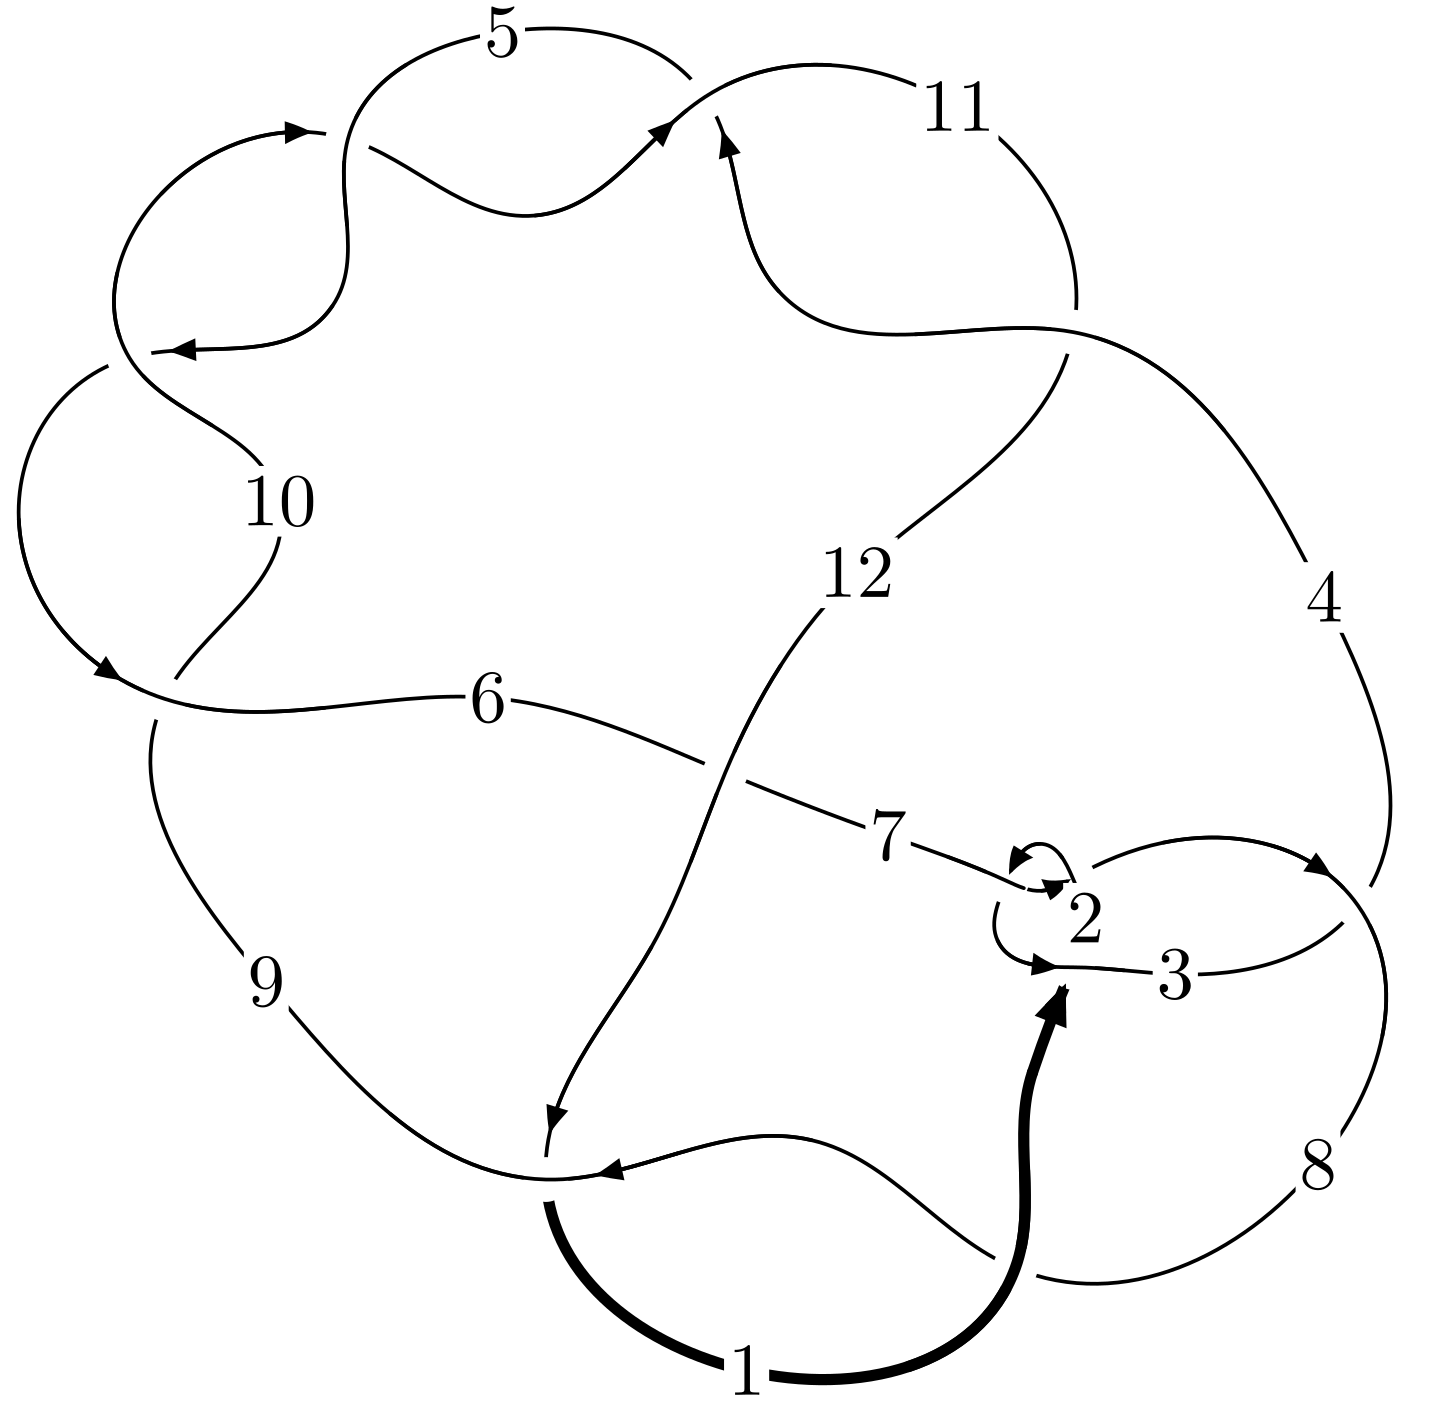
\includegraphics[width=112pt]{../../../GIT/diagram.site/Diagrams/png/1352_12a_0551.png}\\
\ \ \ A knot diagram\footnotemark}&
\allowdisplaybreaks
\textbf{Linearized knot diagam} \\
\cline{2-2}
 &
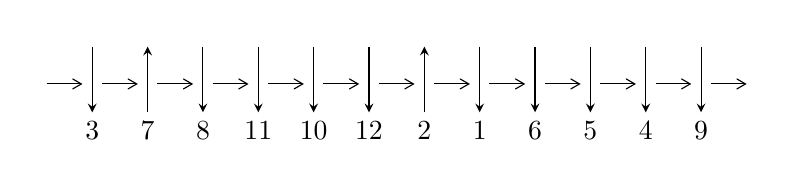
\begin{tikzpicture}[x=20pt, y=17pt]
	% nodes
	\node (C0) at (0, 0) {};
	\node (C1) at (1, 0) {};
	\node (C1U) at (1, +1) {};
	\node (C1D) at (1, -1) {3};

	\node (C2) at (2, 0) {};
	\node (C2U) at (2, +1) {};
	\node (C2D) at (2, -1) {7};

	\node (C3) at (3, 0) {};
	\node (C3U) at (3, +1) {};
	\node (C3D) at (3, -1) {8};

	\node (C4) at (4, 0) {};
	\node (C4U) at (4, +1) {};
	\node (C4D) at (4, -1) {11};

	\node (C5) at (5, 0) {};
	\node (C5U) at (5, +1) {};
	\node (C5D) at (5, -1) {10};

	\node (C6) at (6, 0) {};
	\node (C6U) at (6, +1) {};
	\node (C6D) at (6, -1) {12};

	\node (C7) at (7, 0) {};
	\node (C7U) at (7, +1) {};
	\node (C7D) at (7, -1) {2};

	\node (C8) at (8, 0) {};
	\node (C8U) at (8, +1) {};
	\node (C8D) at (8, -1) {1};

	\node (C9) at (9, 0) {};
	\node (C9U) at (9, +1) {};
	\node (C9D) at (9, -1) {6};

	\node (C10) at (10, 0) {};
	\node (C10U) at (10, +1) {};
	\node (C10D) at (10, -1) {5};

	\node (C11) at (11, 0) {};
	\node (C11U) at (11, +1) {};
	\node (C11D) at (11, -1) {4};

	\node (C12) at (12, 0) {};
	\node (C12U) at (12, +1) {};
	\node (C12D) at (12, -1) {9};
	\node (C13) at (13, 0) {};

	% arrows
	\draw[->,>={angle 60}]
	(C0) edge (C1) (C1) edge (C2) (C2) edge (C3) (C3) edge (C4) (C4) edge (C5) (C5) edge (C6) (C6) edge (C7) (C7) edge (C8) (C8) edge (C9) (C9) edge (C10) (C10) edge (C11) (C11) edge (C12) (C12) edge (C13) ;	\draw[->,>=stealth]
	(C1U) edge (C1D) (C2D) edge (C2U) (C3U) edge (C3D) (C4U) edge (C4D) (C5U) edge (C5D) (C6U) edge (C6D) (C7D) edge (C7U) (C8U) edge (C8D) (C9U) edge (C9D) (C10U) edge (C10D) (C11U) edge (C11D) (C12U) edge (C12D) ;
	\end{tikzpicture} \\
\hhline{~~} \\& 
\textbf{Solving Sequence} \\ \cline{2-2} 
 &
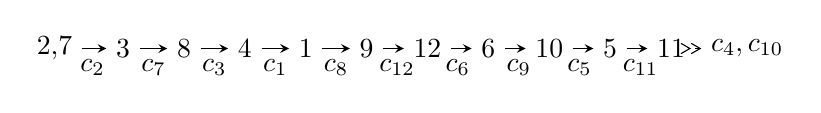
\begin{tikzpicture}[x=22pt, y=7pt]
	% node
	\node (A0) at (-1/8, 0) {2,7};
	\node (A1) at (1, 0) {3};
	\node (A2) at (2, 0) {8};
	\node (A3) at (3, 0) {4};
	\node (A4) at (4, 0) {1};
	\node (A5) at (5, 0) {9};
	\node (A6) at (6, 0) {12};
	\node (A7) at (7, 0) {6};
	\node (A8) at (8, 0) {10};
	\node (A9) at (9, 0) {5};
	\node (A10) at (10, 0) {11};
	\node (C1) at (1/2, -1) {$c_{2}$};
	\node (C2) at (3/2, -1) {$c_{7}$};
	\node (C3) at (5/2, -1) {$c_{3}$};
	\node (C4) at (7/2, -1) {$c_{1}$};
	\node (C5) at (9/2, -1) {$c_{8}$};
	\node (C6) at (11/2, -1) {$c_{12}$};
	\node (C7) at (13/2, -1) {$c_{6}$};
	\node (C8) at (15/2, -1) {$c_{9}$};
	\node (C9) at (17/2, -1) {$c_{5}$};
	\node (C10) at (19/2, -1) {$c_{11}$};
	\node (A11) at (45/4, 0) {$c_{4},c_{10}$};

	% edge
	\draw[->,>=stealth]	
	(A0) edge (A1) (A1) edge (A2) (A2) edge (A3) (A3) edge (A4) (A4) edge (A5) (A5) edge (A6) (A6) edge (A7) (A7) edge (A8) (A8) edge (A9) (A9) edge (A10) ;
	\draw[->>,>={angle 60}]	
	(A10) edge (A11);
\end{tikzpicture} \\ 

\end{tabular} \\

\footnotetext{
The image of knot diagram is generated by the software ``\textbf{Draw programme}" developed by Andrew Bartholomew(\url{http://www.layer8.co.uk/maths/draw/index.htm\#Running-draw}), where we modified some parts for our purpose(\url{https://github.com/CATsTAILs/LinksPainter}).
}\phantom \\ \newline 
\centering \textbf{Ideals for irreducible components\footnotemark of $X_{\text{par}}$} 
 
\begin{align*}
I^u_{1}&=\langle 
u^{51}- u^{50}+\cdots+2 u-1\rangle \\
\\
\end{align*}
\raggedright * 1 irreducible components of $\dim_{\mathbb{C}}=0$, with total 51 representations.\\
\footnotetext{All coefficients of polynomials are rational numbers. But the coefficients are sometimes approximated in decimal forms when there is not enough margin.}
\newpage
\renewcommand{\arraystretch}{1}
\centering \section*{I. $I^u_{1}= \langle u^{51}- u^{50}+\cdots+2 u-1 \rangle$}
\flushleft \textbf{(i) Arc colorings}\\
\begin{tabular}{m{7pt} m{180pt} m{7pt} m{180pt} }
\flushright $a_{2}=$&$\begin{pmatrix}1\\0\end{pmatrix}$ \\
\flushright $a_{7}=$&$\begin{pmatrix}0\\u\end{pmatrix}$ \\
\flushright $a_{3}=$&$\begin{pmatrix}1\\- u^2\end{pmatrix}$ \\
\flushright $a_{8}=$&$\begin{pmatrix}u\\u\end{pmatrix}$ \\
\flushright $a_{4}=$&$\begin{pmatrix}u^4+u^2+1\\u^4\end{pmatrix}$ \\
\flushright $a_{1}=$&$\begin{pmatrix}u^2+1\\- u^4\end{pmatrix}$ \\
\flushright $a_{9}=$&$\begin{pmatrix}- u^7-2 u^5-2 u^3\\u^9+u^7+u^5+u\end{pmatrix}$ \\
\flushright $a_{12}=$&$\begin{pmatrix}u^{12}+3 u^{10}+5 u^8+4 u^6+2 u^4+u^2+1\\- u^{14}-2 u^{12}-3 u^{10}-2 u^8-2 u^6-2 u^4- u^2\end{pmatrix}$ \\
\flushright $a_{6}=$&$\begin{pmatrix}u^{25}+6 u^{23}+\cdots+2 u^3+u\\- u^{27}-5 u^{25}+\cdots- u^3+u\end{pmatrix}$ \\
\flushright $a_{10}=$&$\begin{pmatrix}- u^{43}-10 u^{41}+\cdots-8 u^5-3 u^3\\u^{45}+9 u^{43}+\cdots- u^3+u\end{pmatrix}$ \\
\flushright $a_{5}=$&$\begin{pmatrix}u^{40}+9 u^{38}+\cdots-3 u^4+1\\u^{40}+8 u^{38}+\cdots+6 u^6+2 u^4\end{pmatrix}$ \\
\flushright $a_{11}=$&$\begin{pmatrix}- u^{22}-5 u^{20}+\cdots-3 u^4+1\\- u^{22}-4 u^{20}+\cdots-2 u^4- u^2\end{pmatrix}$\\&\end{tabular}
\flushleft \textbf{(ii) Obstruction class $= -1$}\\~\\
\flushleft \textbf{(iii) Cusp Shapes $= 4 u^{49}-4 u^{48}+\cdots+4 u-14$}\\~\\
\newpage\renewcommand{\arraystretch}{1}
\flushleft \textbf{(iv) u-Polynomials at the component}\newline \\
\begin{tabular}{m{50pt}|m{274pt}}
Crossings & \hspace{64pt}u-Polynomials at each crossing \\
\hline $$\begin{aligned}c_{1}\end{aligned}$$&$\begin{aligned}
&u^{51}+23 u^{50}+\cdots+2 u-1
\end{aligned}$\\
\hline $$\begin{aligned}c_{2},c_{7}\end{aligned}$$&$\begin{aligned}
&u^{51}+u^{50}+\cdots+2 u+1
\end{aligned}$\\
\hline $$\begin{aligned}c_{3}\end{aligned}$$&$\begin{aligned}
&u^{51}- u^{50}+\cdots-4 u+1
\end{aligned}$\\
\hline $$\begin{aligned}c_{4},c_{5},c_{9}\\c_{10},c_{11}\end{aligned}$$&$\begin{aligned}
&u^{51}+u^{50}+\cdots+4 u+1
\end{aligned}$\\
\hline $$\begin{aligned}c_{6}\end{aligned}$$&$\begin{aligned}
&u^{51}+u^{50}+\cdots+4596 u+2061
\end{aligned}$\\
\hline $$\begin{aligned}c_{8},c_{12}\end{aligned}$$&$\begin{aligned}
&u^{51}+5 u^{50}+\cdots+26 u+7
\end{aligned}$\\
\hline
\end{tabular}\\~\\
\newpage\renewcommand{\arraystretch}{1}
\flushleft \textbf{(v) Riley Polynomials at the component}\newline \\
\begin{tabular}{m{50pt}|m{274pt}}
Crossings & \hspace{64pt}Riley Polynomials at each crossing \\
\hline $$\begin{aligned}c_{1}\end{aligned}$$&$\begin{aligned}
&y^{51}+11 y^{50}+\cdots+26 y-1
\end{aligned}$\\
\hline $$\begin{aligned}c_{2},c_{7}\end{aligned}$$&$\begin{aligned}
&y^{51}+23 y^{50}+\cdots+2 y-1
\end{aligned}$\\
\hline $$\begin{aligned}c_{3}\end{aligned}$$&$\begin{aligned}
&y^{51}- y^{50}+\cdots+50 y-1
\end{aligned}$\\
\hline $$\begin{aligned}c_{4},c_{5},c_{9}\\c_{10},c_{11}\end{aligned}$$&$\begin{aligned}
&y^{51}+67 y^{50}+\cdots+2 y-1
\end{aligned}$\\
\hline $$\begin{aligned}c_{6}\end{aligned}$$&$\begin{aligned}
&y^{51}+27 y^{50}+\cdots-54758682 y-4247721
\end{aligned}$\\
\hline $$\begin{aligned}c_{8},c_{12}\end{aligned}$$&$\begin{aligned}
&y^{51}+43 y^{50}+\cdots-1634 y-49
\end{aligned}$\\
\hline
\end{tabular}\\~\\
\newpage\flushleft \textbf{(vi) Complex Volumes and Cusp Shapes}
$$\begin{array}{c|c|c}  
\text{Solutions to }I^u_{1}& \I (\text{vol} + \sqrt{-1}CS) & \text{Cusp shape}\\
 \hline 
\begin{aligned}
u &= \phantom{-}0.124050 + 1.007820 I\end{aligned}
 & -1.22807 - 1.23128 I & -11.11038 + 4.31437 I \\ \hline\begin{aligned}
u &= \phantom{-}0.124050 - 1.007820 I\end{aligned}
 & -1.22807 + 1.23128 I & -11.11038 - 4.31437 I \\ \hline\begin{aligned}
u &= -0.567657 + 0.794330 I\end{aligned}
 & \phantom{-}13.08480 - 2.27933 I & \phantom{-}0.58371 + 3.39997 I \\ \hline\begin{aligned}
u &= -0.567657 - 0.794330 I\end{aligned}
 & \phantom{-}13.08480 + 2.27933 I & \phantom{-}0.58371 - 3.39997 I \\ \hline\begin{aligned}
u &= \phantom{-}0.491070 + 0.796347 I\end{aligned}
 & \phantom{-}3.39837 + 2.06094 I & \phantom{-}0.34753 - 4.06473 I \\ \hline\begin{aligned}
u &= \phantom{-}0.491070 - 0.796347 I\end{aligned}
 & \phantom{-}3.39837 - 2.06094 I & \phantom{-}0.34753 + 4.06473 I \\ \hline\begin{aligned}
u &= -0.764672 + 0.536054 I\end{aligned}
 & \phantom{-}18.2452 - 4.1032 I & \phantom{-}1.95310 + 2.72318 I \\ \hline\begin{aligned}
u &= -0.764672 - 0.536054 I\end{aligned}
 & \phantom{-}18.2452 + 4.1032 I & \phantom{-}1.95310 - 2.72318 I \\ \hline\begin{aligned}
u &= -0.275626 + 0.885976 I\end{aligned}
 & -0.65991 - 1.25740 I & -7.37275 + 5.16821 I \\ \hline\begin{aligned}
u &= -0.275626 - 0.885976 I\end{aligned}
 & -0.65991 + 1.25740 I & -7.37275 - 5.16821 I \\ \hline\begin{aligned}
u &= -0.095918 + 1.079980 I\end{aligned}
 & \phantom{-}2.64743 + 3.72333 I & -5.51914 - 4.10632 I \\ \hline\begin{aligned}
u &= -0.095918 - 1.079980 I\end{aligned}
 & \phantom{-}2.64743 - 3.72333 I & -5.51914 + 4.10632 I \\ \hline\begin{aligned}
u &= \phantom{-}0.748117 + 0.519457 I\end{aligned}
 & \phantom{-}8.20876 + 2.78699 I & \phantom{-}1.43171 - 3.73896 I \\ \hline\begin{aligned}
u &= \phantom{-}0.748117 - 0.519457 I\end{aligned}
 & \phantom{-}8.20876 - 2.78699 I & \phantom{-}1.43171 + 3.73896 I \\ \hline\begin{aligned}
u &= \phantom{-}0.796612 + 0.437292 I\end{aligned}
 & \phantom{-}17.6940 - 7.1625 I & \phantom{-}1.28660 + 3.00306 I \\ \hline\begin{aligned}
u &= \phantom{-}0.796612 - 0.437292 I\end{aligned}
 & \phantom{-}17.6940 + 7.1625 I & \phantom{-}1.28660 - 3.00306 I \\ \hline\begin{aligned}
u &= -0.778283 + 0.440419 I\end{aligned}
 & \phantom{-}7.77323 + 5.65959 I & \phantom{-}0.63336 - 4.31014 I \\ \hline\begin{aligned}
u &= -0.778283 - 0.440419 I\end{aligned}
 & \phantom{-}7.77323 - 5.65959 I & \phantom{-}0.63336 + 4.31014 I \\ \hline\begin{aligned}
u &= -0.371193 + 1.043920 I\end{aligned}
 & -1.29263 - 0.95577 I & -8.94786 - 0.46472 I \\ \hline\begin{aligned}
u &= -0.371193 - 1.043920 I\end{aligned}
 & -1.29263 + 0.95577 I & -8.94786 + 0.46472 I \\ \hline\begin{aligned}
u &= \phantom{-}0.091632 + 1.113570 I\end{aligned}
 & \phantom{-}12.41680 - 5.09230 I & -4.77006 + 2.62305 I \\ \hline\begin{aligned}
u &= \phantom{-}0.091632 - 1.113570 I\end{aligned}
 & \phantom{-}12.41680 + 5.09230 I & -4.77006 - 2.62305 I \\ \hline\begin{aligned}
u &= -0.730042 + 0.483625 I\end{aligned}
 & \phantom{-}3.79742 - 0.31118 I & -2.99375 + 3.59553 I \\ \hline\begin{aligned}
u &= -0.730042 - 0.483625 I\end{aligned}
 & \phantom{-}3.79742 + 0.31118 I & -2.99375 - 3.59553 I \\ \hline\begin{aligned}
u &= \phantom{-}0.748991 + 0.449203 I\end{aligned}
 & \phantom{-}3.60271 - 2.92364 I & -3.83628 + 4.17852 I \\ \hline\begin{aligned}
u &= \phantom{-}0.748991 - 0.449203 I\end{aligned}
 & \phantom{-}3.60271 + 2.92364 I & -3.83628 - 4.17852 I \\ \hline\begin{aligned}
u &= \phantom{-}0.330853 + 1.087020 I\end{aligned}
 & \phantom{-}7.29518 + 0.30876 I & -8.00000 - 0.78025 I \\ \hline\begin{aligned}
u &= \phantom{-}0.330853 - 1.087020 I\end{aligned}
 & \phantom{-}7.29518 - 0.30876 I & -8.00000 + 0.78025 I \\ \hline\begin{aligned}
u &= \phantom{-}0.431459 + 1.058770 I\end{aligned}
 & -3.31703 + 3.41847 I & -14.6084 - 5.2638 I \\ \hline\begin{aligned}
u &= \phantom{-}0.431459 - 1.058770 I\end{aligned}
 & -3.31703 - 3.41847 I & -14.6084 + 5.2638 I\\
 \hline 
 \end{array}$$\newpage$$\begin{array}{c|c|c}  
\text{Solutions to }I^u_{1}& \I (\text{vol} + \sqrt{-1}CS) & \text{Cusp shape}\\
 \hline 
\begin{aligned}
u &= -0.471802 + 1.075960 I\end{aligned}
 & -0.59913 - 5.95166 I & -8.00000 + 8.50499 I \\ \hline\begin{aligned}
u &= -0.471802 - 1.075960 I\end{aligned}
 & -0.59913 + 5.95166 I & -8.00000 - 8.50499 I \\ \hline\begin{aligned}
u &= \phantom{-}0.490778 + 1.100730 I\end{aligned}
 & \phantom{-}8.34808 + 7.02798 I & -8.00000 - 6.50051 I \\ \hline\begin{aligned}
u &= \phantom{-}0.490778 - 1.100730 I\end{aligned}
 & \phantom{-}8.34808 - 7.02798 I & -8.00000 + 6.50051 I \\ \hline\begin{aligned}
u &= \phantom{-}0.614197 + 1.047040 I\end{aligned}
 & \phantom{-}6.63961 + 2.38883 I & \phantom{-0.000000 } 0 \\ \hline\begin{aligned}
u &= \phantom{-}0.614197 - 1.047040 I\end{aligned}
 & \phantom{-}6.63961 - 2.38883 I & \phantom{-0.000000 } 0 \\ \hline\begin{aligned}
u &= -0.629234 + 1.042400 I\end{aligned}
 & \phantom{-}16.7365 - 1.1689 I & \phantom{-0.000000 } 0 \\ \hline\begin{aligned}
u &= -0.629234 - 1.042400 I\end{aligned}
 & \phantom{-}16.7365 + 1.1689 I & \phantom{-0.000000 } 0 \\ \hline\begin{aligned}
u &= -0.595770 + 1.063400 I\end{aligned}
 & \phantom{-}2.07756 - 4.75365 I & -8.00000 + 0. I\phantom{ +0.000000I} \\ \hline\begin{aligned}
u &= -0.595770 - 1.063400 I\end{aligned}
 & \phantom{-}2.07756 + 4.75365 I & -8.00000 + 0. I\phantom{ +0.000000I} \\ \hline\begin{aligned}
u &= \phantom{-}0.597475 + 1.082780 I\end{aligned}
 & \phantom{-}1.72685 + 8.04071 I & \phantom{-0.000000 } 0 \\ \hline\begin{aligned}
u &= \phantom{-}0.597475 - 1.082780 I\end{aligned}
 & \phantom{-}1.72685 - 8.04071 I & \phantom{-0.000000 } 0 \\ \hline\begin{aligned}
u &= -0.606769 + 1.094070 I\end{aligned}
 & \phantom{-}5.83091 - 10.88290 I & \phantom{-0.000000 } 0 \\ \hline\begin{aligned}
u &= -0.606769 - 1.094070 I\end{aligned}
 & \phantom{-}5.83091 + 10.88290 I & \phantom{-0.000000 } 0 \\ \hline\begin{aligned}
u &= \phantom{-}0.613048 + 1.101110 I\end{aligned}
 & \phantom{-}15.7156 + 12.4555 I & \phantom{-0.000000 } 0 \\ \hline\begin{aligned}
u &= \phantom{-}0.613048 - 1.101110 I\end{aligned}
 & \phantom{-}15.7156 - 12.4555 I & \phantom{-0.000000 } 0 \\ \hline\begin{aligned}
u &= \phantom{-}0.638692 + 0.195238 I\end{aligned}
 & \phantom{-}10.86370 - 2.72758 I & -2.02598 + 2.69670 I \\ \hline\begin{aligned}
u &= \phantom{-}0.638692 - 0.195238 I\end{aligned}
 & \phantom{-}10.86370 + 2.72758 I & -2.02598 - 2.69670 I \\ \hline\begin{aligned}
u &= -0.546991 + 0.180701 I\end{aligned}
 & \phantom{-}1.78156 + 1.95178 I & -2.96735 - 4.57785 I \\ \hline\begin{aligned}
u &= -0.546991 - 0.180701 I\end{aligned}
 & \phantom{-}1.78156 - 1.95178 I & -2.96735 + 4.57785 I \\ \hline\begin{aligned}
u &= \phantom{-}0.433964\phantom{ +0.000000I}\end{aligned}
 & -0.812863\phantom{ +0.000000I} & -12.4030\phantom{ +0.000000I}\\
 \hline 
 \end{array}$$\newpage
\newpage\renewcommand{\arraystretch}{1}
\centering \section*{ II. u-Polynomials}
\begin{tabular}{m{50pt}|m{274pt}}
Crossings & \hspace{64pt}u-Polynomials at each crossing \\
\hline $$\begin{aligned}c_{1}\end{aligned}$$&$\begin{aligned}
&u^{51}+23 u^{50}+\cdots+2 u-1
\end{aligned}$\\
\hline $$\begin{aligned}c_{2},c_{7}\end{aligned}$$&$\begin{aligned}
&u^{51}+u^{50}+\cdots+2 u+1
\end{aligned}$\\
\hline $$\begin{aligned}c_{3}\end{aligned}$$&$\begin{aligned}
&u^{51}- u^{50}+\cdots-4 u+1
\end{aligned}$\\
\hline $$\begin{aligned}c_{4},c_{5},c_{9}\\c_{10},c_{11}\end{aligned}$$&$\begin{aligned}
&u^{51}+u^{50}+\cdots+4 u+1
\end{aligned}$\\
\hline $$\begin{aligned}c_{6}\end{aligned}$$&$\begin{aligned}
&u^{51}+u^{50}+\cdots+4596 u+2061
\end{aligned}$\\
\hline $$\begin{aligned}c_{8},c_{12}\end{aligned}$$&$\begin{aligned}
&u^{51}+5 u^{50}+\cdots+26 u+7
\end{aligned}$\\
\hline
\end{tabular}\newpage\renewcommand{\arraystretch}{1}
\centering \section*{ III. Riley Polynomials}
\begin{tabular}{m{50pt}|m{274pt}}
Crossings & \hspace{64pt}Riley Polynomials at each crossing \\
\hline $$\begin{aligned}c_{1}\end{aligned}$$&$\begin{aligned}
&y^{51}+11 y^{50}+\cdots+26 y-1
\end{aligned}$\\
\hline $$\begin{aligned}c_{2},c_{7}\end{aligned}$$&$\begin{aligned}
&y^{51}+23 y^{50}+\cdots+2 y-1
\end{aligned}$\\
\hline $$\begin{aligned}c_{3}\end{aligned}$$&$\begin{aligned}
&y^{51}- y^{50}+\cdots+50 y-1
\end{aligned}$\\
\hline $$\begin{aligned}c_{4},c_{5},c_{9}\\c_{10},c_{11}\end{aligned}$$&$\begin{aligned}
&y^{51}+67 y^{50}+\cdots+2 y-1
\end{aligned}$\\
\hline $$\begin{aligned}c_{6}\end{aligned}$$&$\begin{aligned}
&y^{51}+27 y^{50}+\cdots-54758682 y-4247721
\end{aligned}$\\
\hline $$\begin{aligned}c_{8},c_{12}\end{aligned}$$&$\begin{aligned}
&y^{51}+43 y^{50}+\cdots-1634 y-49
\end{aligned}$\\
\hline
\end{tabular}
\vskip 2pc
\end{document}